A {\em time series} is a time-ordered sequence of data points. Time series are ubiquitous in many application domains. They can represent various types of measurements, such as user check-ins at various Points of Interest, energy consumption in smart buildings, PM2.5 particle concentration measured by air pollution sensors, etc. Analyzing and mining time series data is highly important for discovering trends and patterns in such phenomena, and has attracted extensive research interest over the last years \cite{DBLP:journals/pvldb/EchihabiZPB18,DBLP:conf/sigmod/LinardiZPK18a,DBLP:journals/datamine/YehZUBDDZSMK18}.

%The time series literature, however, typically overlooks the fact 
However, what is usually overlooked is that the phenomena represented by time series are often also associated with geographic locations, e.g., time series generated by sensors installed at fixed positions. In such cases, spatial distance also plays an important role in the analysis, since discovery of trends and patterns may depend not only on time series similarity but also on geographic proximity. Motivated by this observation, in previous work \cite{chatzig17btsr, DBLP:conf/gis/Chatzigeorgakidis18} we introduced the concept of {\em geolocated} time series and we  proposed hybrid indexing techniques that efficiently support the retrieval of time series based on both spatial distance and time series similarity.

In particular, we introduced the \btsr \cite{chatzig17btsr}, a {\em hybrid index} that first builds an R-tree over the locations of the time series data. It then enhances each node with appropriate upper- and lower-bounding time series (MBTS) that enclose the subset of time series represented by it. Combining MBTSs and MBRs, the query evaluation algorithm can simultaneously prune the search space based on time series similarity and spatial distance while traversing the index. To further increase its pruning power, the \btsr groups together similar time series within each node to derive tighter bounds.

This existing approach for hybrid search over geolocated time series using the \btsr supports only {\em global} time series similarity, i.e., similarity measured across the entire length of time series. Specifically, as in other works in this area \cite{DBLP:journals/pvldb/EchihabiZPB18,jessica2007dmkd,camerra2010icdm,camerra2014kais}, the distance between two time series is measured by aggregating the pairwise Euclidean distance of their respective values across the entire sequences. However, in many cases, more fine-grained trends and patterns may exist, which are missed under this global similarity measure. For example, consider two time series representing the hourly energy consumption of two nearby buildings over a week, and assume that the two buildings exhibit a similar consumption pattern during working days but a different one in weekends. A query imposing a similarity threshold over the entire week would fail to identify these two geolocated time series as similar. However, it may be useful to discover that there is a period of up to 5 days during which these two time series are actually similar.

% \checknote{{\bf Mentioning $\delta$ may be removed from this sentence?} Instead, relaxing this constraint to capture similarities over some time period $\delta$ less than the series length, could identify those two time series as matching for a maximum duration $\delta$ of 5 days.}

%Motivated by this observation, in this work we extend our previous approach on hybrid queries over geolocated time series to support {\em local similarity} of time series, thus allowing more flexible and fine-grained queries and analyses. First, we introduce our criterion for local similarity, which is based on two parameters, $\delta$ and $\epsilon$. The first specifies the minimum length of the subsequences that are required to be similar. The second specifies the maximum difference between the respective values of the time series in order to qualify as matching. Thus, two time series are considered to be locally similar, with respect to $\delta$ and $\epsilon$, if there exist at least $\delta$ consecutive timestamps during which their values do not differ by more than $\epsilon$. Notice that the second condition is stricter than the aggregate Euclidean distance used in the definition of global similarity. The reason is that since we relax the global similarity constraint to allow for local similarity between shorter subsequences, we want to ensure that these subsequences are sufficiently close to each other at each individual timestamp.

Motivated by this observation, in this work we extend our previous approach on hybrid queries over geolocated time series to support {\em local similarity} of time series, thus allowing more flexible and fine-grained queries and analyses.
% To detect such similarities, a parameter $\epsilon$ on the time series domain specifies the maximum difference allowed between the respective values of two time series in order to consider them as similar. Then, a {\em local similarity score} $\delta$ represents the maximum number of consecutive timestamps where their respective values differ by at most $\epsilon$.
The {\em local similarity score} between two time series $T_i$ and $T_j$ is defined as the maximum number of consecutive timestamps during which the respective values of $T_i$ and $T_j$ do not differ by more than a user-specified threshold $\epsilon$.
Notice that, compared to global similarity, this condition is more relaxed, in the sense that it is applied to subsequences of length lower than $T_i$ and $T_j$, but at the same time stricter, in the sense that the threshold $\epsilon$ is required to be satisfied at each individual timestamp during the selected period rather than on the aggregate distance over all timestamps.
% is stricter than the one applied in the case of global similarity
% aggregate Euclidean distance used in establishing global similarity. Indeed, since we relax the global similarity constraint to allow for local similarity between subsequences, we want to ensure that these subsequences are sufficiently close to each other at each individual timestamp.
% \checknote{This local similarity constraint is also coupled with a {\em spatial} predicate (i.e., range or $k$-nearest neighbor), leading to a novel set of hybrid queries. Figure~\ref{fig:example_query} illustrates an example with a query time series $T_q$ searching over a set of time series $\{T_1,\dots,T_9\}$ for those that are within radius $\rho$ from its location and their values deviate by less than $\epsilon$ from $T_q$ across some time interval. A cutoff threshold $\delta$ may be applied to filter out results of low local similarity scores. Qualifying results include $T_2$ with score $\delta_2$ (bottom chart), and $T_7$ with score $\delta_7$ (top chart). Note that $T_7$ is locally similar to $T_q$ also at their termination, but the score concerns the maximum interval among pairwise matches.}

Combining this local similarity constraint with a filter on {\em spatial distance} leads to a novel set of hybrid queries. Figure~\ref{fig:example_query} shows an example with a query time series $T_q$ searching over a set of time series $T_1,\dots,T_9$ for those within radius $\rho$ from its location and also locally similar to $T_q$. In particular, with respect to a given $\epsilon$, results should also be locally similar to $T_q$ for at least 5 consecutive timestamps. Qualifying results include $T_2$ with local similarity score $\sigma_2 = 5$ (bottom chart), and $T_7$ with $\sigma_7 = 7$ (top chart).
% Note that $T_7$ is locally similar to $T_q$ also at their termination, but the score concerns the maximum interval among pairwise matches.

% \checknote{In the Figure, the symbol for time series is $T$. But in the description of the algorithms is $X$. Choose one of them, e.g., $X$ to avoid changing the algorithms?}

% \checknote{KP: I would suggest to use symbols $\rho$ and $\epsilon$ instead of $\epsilon_{sp}$ and $\epsilon_{ts}$. It simplifies presentation and avoids confusion.}

\begin{figure}[!t]
 \centering
 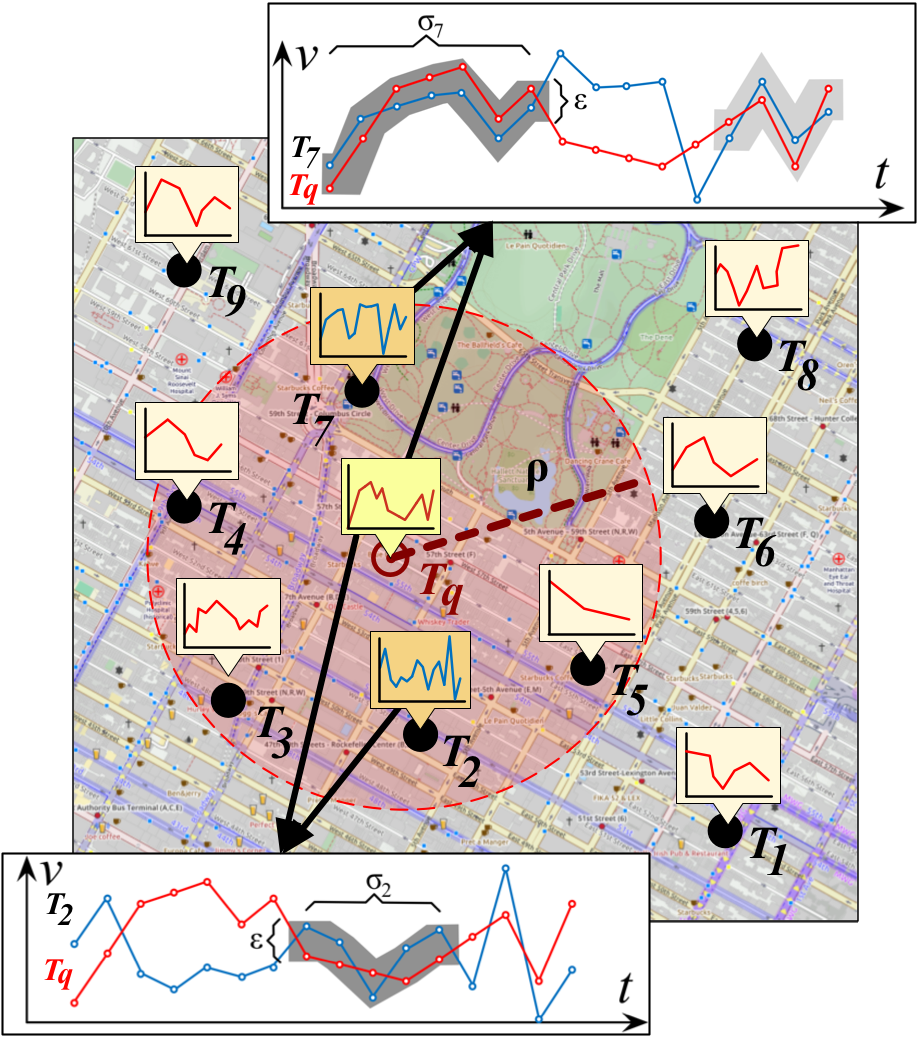
\includegraphics[width=75mm]{Figures/local_sim_geoloc.png}
\caption{Retrieving geolocated time series based on spatial distance and local similarity.}
\label{fig:example_query}
\end{figure}

%Having defined hybrid queries for geolocated time series with local similarity

It turns out that such hybrid queries involving local similarity can still be evaluated using the \btsr index. We first present a baseline method employing a sweep-line algorithm to check for local similarity, and then describe how this can be optimized by using appropriately placed {\em checkpoints}, based on the local similarity score threshold specified by the query, in order to skip unnecessary comparisons. Despite the fact that this saves some computations, the resulting time savings are relatively small, since the number of index nodes that need to be probed is not essentially reduced. To overcome this problem, we introduce an improvement to the \btsr index, which is based on temporally segmenting the time series bounds within each node and deriving tighter bounds per segment. Once the time series bounds in each node become more fine-grained, pruning the search space for local similarity queries proves much more effective.

Summarizing, our main contributions are as follows:

\begin{itemize}
 \item We extend our previous work on hybrid queries for geolocated time series to support local time series similarity. We consider both range and top-$k$ queries, including combined criteria for spatial distance and local time series distance.
 \item We present how such queries can be answered efficiently exploiting the previously introduced \btsr index.
 \item To achieve greater savings in execution time by further reducing node accesses, we propose an enhanced variant of \btsr, called \sbtsr, which additionally employs temporal segmentation in each node to derive tighter, more fine-grained time series bounds.
 \item We experimentally evaluate our methods using real-world datasets from different application domains, showing that \btsr can efficiently handle hybrid queries under local similarity search, while \sbtsr achieves even higher performance due to the additional temporal segmentation.
\end{itemize}

The remainder of the paper is structured as follows. Section \ref{sec:related} reviews related work. Section \ref{sec:problem} formally defines the problem. Section \ref{sec:ls_q_btsr} presents how query evaluation under local time series similarity can be executed using the \btsr, while Section \ref{sec:sbtsr_index} presents the enhanced \sbtsr. Section \ref{sec:exp} reports our experimental results, and Section \ref{sec:conclusions} concludes the paper.


% \checknote{
% Time series are important in many applications, ranging from the Web to finance and biology. Indexing and mining time series data has attracted a lot of interest, both from the database and data mining communities \cite{camerra2014kais,ding2008pvldb,shieh2008kdd}. Nevertheless, support for \emph{geolocated} time series is still lacking. Geolocated time series are time series that are produced at, or otherwise associated with, specific locations.

% Geolocated time series are encountered in numerous applications. In geosocial networks, user check-ins associate locations with time series representing the number of visitors across time. In geomarketing or mobile advertisement, geolocated time series can be used to identify nearby places with similar visiting patterns. Geolocated time series are also generated by geotagged user posts, photos, micropayments, etc. Other examples involve time series generated by sensors installed at fixed locations, such as noise, weather or pollution sensors. In the \textit{DAIAD} project\footnote{\url{http://daiad.eu/}}, smart water meters are installed at households within a city to measure, analyze and mine water consumption patterns towards promoting more intelligent and efficient water use. Finding households in a region or close to a given location that exhibit consumption patterns similar to a given one can offer precious insights.

% All such applications need to index geolocated time series to allow efficient similarity search based on both {\em spatial proximity} and {\em time series similarity}. Several approaches have been proposed for time series similarity, efficiently indexing large amounts of time series data. One well-studied family of approaches includes wavelet-based methods \cite{chan1999icde}, which rely on \emph{Discrete Wavelet Transform} \cite{graps1995cse} to reduce the dimensionality of time series and generate an index using the coefficients of the transformed sequences. Another line of work employs a \emph{Symbolic Aggregate Approximation} (SAX) representation of time series \cite{jessica2007dmkd}, introducing a series of indices, such as $i$SAX~\cite{shieh2008kdd}, $i$SAX 2.0~\cite{camerra2010icdm}, $i$SAX2+~\cite{camerra2014kais}, and ADS+~\cite{zoumpatianos2014sigmod}.

% However, to the best of our knowledge, none of the existing works so far has considered the specific case of geolocated time series. All aforementioned indices aim at efficiently supporting similarity search for time series; in case that the analyzed time series are associated with a spatial attribute and issued queries involve spatial filters, these need to be treated independently. Thus, for queries employing both types of predicates, this implies evaluating each predicate separately. This can be done by first using  a time series index to retrieve similar time series and then applying the spatial predicate on the results, or vice versa, by employing a spatial index to evaluate the spatial predicate and then filter the results according to their similarity with the query time series.

% In this paper, we propose a {\em hybrid index} for efficiently supporting similarity search on geolocated time series combining both spatial proximity and time series similarity. The proposed index, called \textit{\sbtsr}, is an extension of the R-tree spatial index. In the\sbtsr, each node is augmented with additional information corresponding to the bounds of the time series contained in its subtree, in addition to the standard \emph{Minimum Bounding Rectangle} (MBR) denoting the spatial bound of its contents. Maintaining both kinds of bounds in each node allows to prune the search space simultaneously in the spatial dimension and in the time series dimension while traversing the index. Thus, the number of required node accesses is significantly reduced, since we only retrieve the contents of nodes that may actually contain objects satisfying both types of predicates.

% In addition, we propose an optimized variant, the \textit{\btsr}, with its nodes having entries with more refined bounds by bundling together similar time series. This allows to compute and maintain tighter bounds for each individual bundle, hence increasing pruning effectiveness. To allow for a larger number of bundles in nodes at higher levels in the tree hierarchy, we exploit \emph{Piecewise Aggregate Approximation} \cite{keogh2001paa,faloutsos2000vldb} to trade off between the number of bundles and the resolution of the bounding time series for each bundle.

% Our proposed approach follows a similar rationale to that applied in {\em hybrid spatio-textual indices} \cite{chen2013vldb}. In that line of research, several variants of hybrid indices (e.g., the IR-tree \cite{cong2009vldb}) have been proposed to tackle the problem of combining spatial predicates with keyword search. Constructing a hybrid index that combines spatial and textual pruning has been shown to speedup processing of hybrid spatial-keyword queries. Motivated by this, our goal is to provide similar improvements for queries on geolocated time series data. Nevertheless, spatio-textual indices are designed specifically for keyword search and typically rely on inverted indices for the textual part, hence they are not applicable to queries that involve similarity of time series where the sequence of values is important.

% Summarizing, our main contributions are as follows:

% \begin{itemize}
%  \item We address the problem of similarity search for geolocated time series, via hybrid boolean or top-$k$ queries combining both spatial proximity and time series similarity.
%  \item We propose the \sbtsr, a hybrid index for geolocated time series, extending the spatial R-tree and augmenting each node with appropriate time series bounds.
%  \item We further optimize the \sbtsr to derive a more efficient variant, the \btsr, that clusters the time series of each subtree to derive and maintain tighter bounds for pruning.
%  \item We experimentally validate our proposed approach using real-world datasets from different application use cases, showing that our hybrid indices can effectively allow simultaneous pruning of the search space in both spatial and time series domains, significantly reducing the required number of node accesses.
% \end{itemize}

% The rest of the paper is organized as follows. Section \ref{sec:related} reviews related work. Section \ref{sec:problem} introduces the distance measures and hybrid query variants on geolocated time series data. Sections \ref{sec:ls_q_btsr} and \ref{sec:sbtsr_index} present the \btsr and \sbtsr indices. Section \ref{sec:exp} reports our experimental results, and Section \ref{sec:conclusions} concludes the paper.
% }